% ---------------------------------------------------------------------------
% Diagrama de bloques de un canal del transceptor serie configurable.
% Fuente del PDF que incluye la memoria (capítulo 3).
%
% Compilar:  pdflatex diagrama_transceptor.tex
% ---------------------------------------------------------------------------
\documentclass[border=8pt]{standalone}
\usepackage[utf8]{inputenc}
\usepackage[T1]{fontenc}
\usepackage{lmodern}
\usepackage{tikz}
\usetikzlibrary{arrows.meta, calc}

% Paleta coherente con las gráficas de la memoria
\definecolor{cPropio}{HTML}{2A78D6}   % azul: lógica de diseño propio
\definecolor{cIP}{HTML}{EDA100}       % ámbar: IP de terceros
\definecolor{cExt}{HTML}{1BAF7A}      % aguamarina: fuera de la FPGA
\definecolor{cRef}{HTML}{8A8A85}      % gris: líneas y contornos

\begin{document}
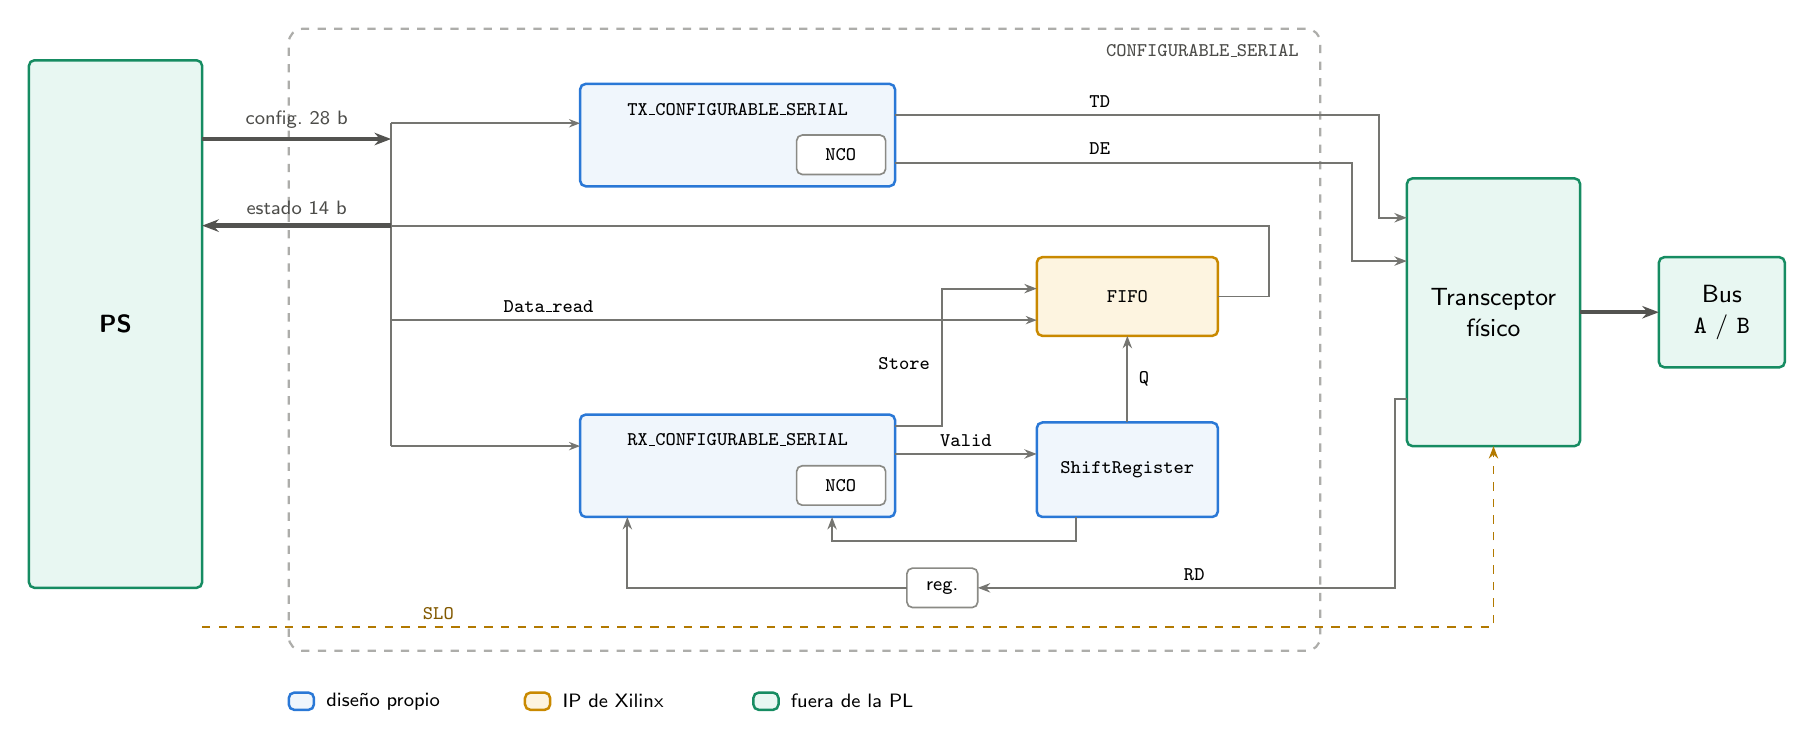
\begin{tikzpicture}[
    x=1cm, y=1cm, font=\sffamily\small,
    blk/.style={draw=cPropio, line width=0.9pt, rounded corners=2pt,
                fill=cPropio!7},
    ip/.style={draw=cIP!85!black, line width=0.9pt, rounded corners=2pt,
               fill=cIP!12},
    ext/.style={draw=cExt!80!black, line width=0.9pt, rounded corners=2pt,
                fill=cExt!10},
    aux/.style={draw=cRef, line width=0.6pt, rounded corners=2pt, fill=white},
    sig/.style={-{Stealth[length=4.5pt]}, line width=0.7pt, cRef!85!black},
    bus/.style={-{Stealth[length=6pt]}, line width=1.6pt, cRef!60!black},
    stub/.style={-{Stealth[length=4pt]}, line width=0.7pt, cRef!85!black},
    lbl/.style={font=\sffamily\scriptsize, inner sep=2pt},
    tlbl/.style={font=\ttfamily\scriptsize, inner sep=2pt},
    name/.style={font=\ttfamily\scriptsize, align=center},
]

% ===================== Envolvente del canal =====================
\draw[draw=cRef!70, dashed, line width=0.8pt, rounded corners=5pt]
      (3.30,0.40) rectangle (16.40,8.30);
\node[name, anchor=north east, text=cRef!55!black] at (16.25,8.22)
      {CONFIGURABLE\_SERIAL};

% ===================== PS =====================
\draw[ext] (0,1.20) rectangle (2.20,7.90);
\node at (1.10,4.55) {\textbf{PS}};

% ===================== Transmisor =====================
\draw[blk] (7.00,6.30) rectangle (11.00,7.60);
\node[name] at (9.00,7.28) {TX\_CONFIGURABLE\_SERIAL};
\draw[aux] (9.75,6.45) rectangle (10.88,6.95);
\node[font=\ttfamily\scriptsize] at (10.31,6.70) {NCO};

% ===================== Receptor =====================
\draw[blk] (7.00,2.10) rectangle (11.00,3.40);
\node[name] at (9.00,3.08) {RX\_CONFIGURABLE\_SERIAL};
\draw[aux] (9.75,2.25) rectangle (10.88,2.75);
\node[font=\ttfamily\scriptsize] at (10.31,2.50) {NCO};

% ===================== Registro de desplazamiento y FIFO =====================
\draw[blk] (12.80,2.10) rectangle (15.10,3.30);
\node[name] at (13.95,2.70) {ShiftRegister};

\draw[ip] (12.80,4.40) rectangle (15.10,5.40);
\node[name] at (13.95,4.90) {FIFO};

% ===================== Registro de la línea de entrada =====================
\draw[aux] (11.15,0.95) rectangle (12.05,1.45);
\node[lbl] at (11.60,1.20) {reg.};

% ===================== Transceptor físico y bus =====================
\draw[ext] (17.50,3.00) rectangle (19.70,6.40);
\node[align=center] at (18.60,4.70) {Transceptor\\físico};
\draw[ext] (20.70,4.00) rectangle (22.30,5.40);
\node[align=center] at (21.50,4.70) {Bus\\\texttt{A} / \texttt{B}};

% ===================== Vector de escritura y configuración =====================
\draw[bus] (2.20,6.90) -- (4.60,6.90);
\node[lbl, above, text=cRef!55!black] at (3.40,6.96) {config.\ 28~b};
\draw[line width=0.7pt, cRef!85!black] (4.60,3.00) -- (4.60,7.10);
\draw[stub] (4.60,7.10) -- (7.00,7.10);
\draw[stub] (4.60,3.00) -- (7.00,3.00);
\draw[stub] (4.60,4.60) -- (12.80,4.60);
\node[tlbl, above] at (6.60,4.62) {\texttt{Data\_read}};

% ===================== Vector de estado y lectura =====================
\draw[line width=0.7pt, cRef!85!black] (15.10,4.90) -- (15.75,4.90)
      -- (15.75,5.80) -- (4.60,5.80);
\draw[bus] (4.60,5.80) -- (2.20,5.80);
\node[lbl, above, text=cRef!55!black] at (3.40,5.86) {estado 14~b};

% ===================== Camino de transmisión =====================
\draw[sig] (11.00,7.20) -- (17.15,7.20) -- (17.15,5.90) -- (17.50,5.90);
\node[tlbl, above] at (13.60,7.22) {\texttt{TD}};
\draw[sig] (11.00,6.60) -- (16.80,6.60) -- (16.80,5.35) -- (17.50,5.35);
\node[tlbl, above] at (13.60,6.62) {\texttt{DE}};

% ===================== Camino de recepción =====================
\draw[sig] (17.50,3.60) -- (17.35,3.60) -- (17.35,1.20) -- (12.05,1.20);
\node[tlbl, above] at (14.80,1.22) {\texttt{RD}};
\draw[sig] (11.15,1.20) -- (7.60,1.20) -- (7.60,2.10);

\draw[sig] (11.00,2.90) -- (12.80,2.90);
\node[tlbl, above] at (11.90,2.92) {\texttt{Valid}};

\draw[sig] (13.95,3.30) -- (13.95,4.40);
\node[tlbl, right] at (14.02,3.85) {\texttt{Q}};

% realimentación de la palabra normalizada hacia el receptor
\draw[sig] (13.30,2.10) -- (13.30,1.80) -- (10.20,1.80) -- (10.20,2.10);

% escritura de la palabra completa en la FIFO
\draw[sig] (11.00,3.25) -- (11.60,3.25) -- (11.60,5.00) -- (12.80,5.00);
\node[tlbl, anchor=east] at (11.52,4.05) {\texttt{Store}};

% ===================== Bus físico =====================
\draw[bus] (19.70,4.70) -- (20.70,4.70);

% ===================== SLO: del vector de configuración al pin =====================
\draw[sig, dashed, cIP!75!black] (2.20,0.70) -- (18.60,0.70) -- (18.60,3.00);
\node[tlbl, above, text=cIP!55!black] at (5.20,0.72) {\texttt{SLO}};

% ===================== Leyenda =====================
\draw[blk] (3.30,-0.35) rectangle (3.62,-0.13);
\node[lbl, anchor=west] at (3.70,-0.24) {diseño propio};
\draw[ip] (6.30,-0.35) rectangle (6.62,-0.13);
\node[lbl, anchor=west] at (6.70,-0.24) {IP de Xilinx};
\draw[ext] (9.20,-0.35) rectangle (9.52,-0.13);
\node[lbl, anchor=west] at (9.60,-0.24) {fuera de la PL};

\end{tikzpicture}
\end{document}
